\section{Proof-of-Concept}
\label{sec:poc}

This section describes the proof-of-concept bot developed to demonstrate and validate recursive leverage mechanics on a real blockchain. The bot operates on Base mainnet using the yoUSD/USDC market on Morpho Blue.

\subsection{Design Goals}

The purpose of the proof-of-concept is to demonstrate recursive leverage mechanics on a live chain before analysing whale behaviour on Ethereum mainnet. The bot validates the looping process end-to-end: depositing capital, supplying collateral, borrowing against it, and repeating the cycle to amplify exposure.

We deploy on Base rather than Ethereum mainnet to minimise gas costs during development and testing. Base is an Ethereum Layer-2 with significantly lower transaction fees while maintaining compatibility with mainnet contracts. The empirical analysis in later sections uses Ethereum mainnet data due to higher capital concentration, deeper liquidity, and longer transaction histories.

We selected yoUSD as the yield-bearing token because it is fully permissionless (no whitelist), implements the ERC-4626 vault standard for simple deposit and redemption, offers approximately 8\% native APY paid in USDC, and has a confirmed Morpho Blue market on Base with 91.5\% liquidation LTV.

Ownership of the deployed contract is transferred to a 1-of-2 Gnosis Safe multisig wallet. This separation of deployment signer and operational signer provides higher security and allows the use of Gnosis Safe's transaction builder for complex operations.

\begin{figure}[h]
\centering
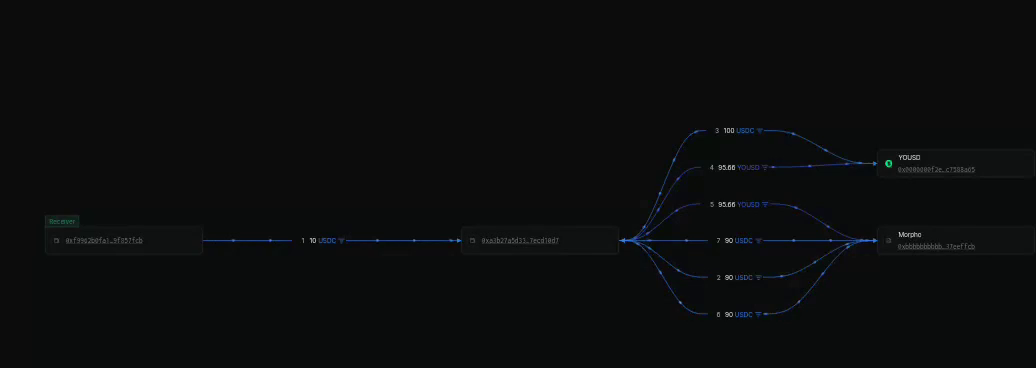
\includegraphics[width=\textwidth]{figures/leverage-flow.png}
\caption{Execution flow of the flashloan-based leverage strategy, visualised via Tenderly.\protect\footnote{\url{https://dashboard.tenderly.co/public/safe/safe-apps/simulator/7fb53629-e928-45d1-830b-9dc967b76ccc/fund-flow}}}
\label{fig:leverage-flow}
\end{figure}

\subsection{Strategy 1: Flashloan-Based Leverage}

The first strategy uses a Morpho flashloan to build the entire leveraged position atomically in a single transaction. This approach is implemented in the \texttt{LeverageBot.sol} smart contract.

The execution flow proceeds as follows:
\begin{enumerate}
    \item The owner approves 10 USDC and calls \texttt{execute()}.
    \item The contract pulls 10 USDC from the owner, then requests a 90 USDC flashloan from Morpho.
    \item Morpho calls back \texttt{onMorphoFlashLoan()}; the contract now holds 100 USDC.
    \item The contract deposits all 100 USDC into the yoUSD vault, receiving approximately 93 yoUSD shares.
    \item The contract supplies yoUSD as collateral on Morpho in the yoUSD/USDC market.
    \item The contract borrows 90 USDC against the yoUSD collateral.
    \item The contract repays the 90 USDC flashloan; the transaction completes.
\end{enumerate}

The result is approximately 100 USDC worth of yoUSD collateral with 90 USDC of debt, funded with only 10 USDC of the owner's capital. This represents roughly 10x leverage.

The \texttt{unwind()} function reverses this process atomically: it flashloans enough USDC to repay the debt, withdraws all yoUSD collateral, redeems yoUSD back to USDC, repays the flashloan, and sweeps any remaining USDC (original capital plus accrued yield) to the owner.

\subsection{Strategy 2: Iterative Looping}

The second strategy requires no smart contract. It uses a JavaScript script that loops step-by-step across multiple transactions:
\begin{enumerate}
    \item Deposit USDC into yoUSD vault, receive yoUSD shares.
    \item Supply yoUSD as collateral on Morpho.
    \item Borrow 88\% of the collateral value back as USDC.
    \item Repeat with the borrowed USDC.
\end{enumerate}

The script executes three loops by default, building up leverage incrementally. If any loop fails, the script automatically triggers \texttt{unwind.js} to clean up the partial position.

This approach is slower (multiple transactions incur multiple gas fees) but simpler to understand and debug. It also demonstrates the manual process that many whale addresses use, as observed in the empirical data.

\subsection{Security Considerations}

Several security measures are implemented:

\textbf{Ownership model.} The contract uses an \texttt{onlyOwner} modifier for privileged functions (\texttt{execute}, \texttt{unwind}, \texttt{rescueToken}). Ownership is transferred to a Gnosis Safe after deployment.

\textbf{Flashloan callback guard.} The \texttt{onMorphoFlashLoan} callback is protected by an \texttt{onlyMorpho} modifier, ensuring only Morpho can invoke it.

\textbf{Rescue function.} A \texttt{rescueToken} function allows the owner to recover any tokens accidentally sent to the contract.

\textbf{Atomic execution.} The flashloan strategy executes entirely within a single transaction. If any step fails, the entire transaction reverts, leaving no partial state.

\subsection{Deployment and Testing}

The contract is deployed on Base mainnet at address \texttt{0xa3B27a...Ecd10d7}, with ownership transferred to a 1-of-2 Gnosis Safe at \texttt{0xf9962B...857fCb}. Full addresses are recorded in the deployment artefacts.

\textbf{Operational workflow.} To execute the leverage strategy via the Safe, the operator uses the Gnosis Safe Transaction Builder:
\begin{enumerate}
    \item Create a new transaction, paste the USDC contract address on Base, and let the interface auto-generate the ABI.
    \item Call \texttt{approve()} with the bot address as spender and 10 USDC as the amount. This is a one-time approval.
    \item Create a second transaction targeting the bot contract and call \texttt{execute()}.
    \item Optionally simulate the transaction via Tenderly to preview the fund flow before signing.
    \item Sign and execute the transaction through the Safe.
\end{enumerate}

The Tenderly simulator provides a visual flowchart animation showing the complete execution path: USDC transfer, flashloan request, yoUSD deposit, collateral supply, borrow, and flashloan repayment (Figure~\ref{fig:leverage-flow}).

\textbf{Testing.} Tests run against a real Base fork using Hardhat, with no mocks or stubs. The test suite covers:
\begin{itemize}
    \item Execution flow and position state verification
    \item Ownership transfer and access control
    \item Unwind functionality and USDC recovery
    \item Flashloan callback guards
    \item Full lifecycle via Safe-impersonated transactions
\end{itemize}

All contract addresses are recorded in \texttt{deployments/LeverageBot\_base\_latest.json}. The full contract code is provided in Appendix~\ref{sec:code}.
